\documentclass[a4paper, 12pt]{article}%тип документа

%отступы
\usepackage[left=2cm,right=2cm,top=2cm,bottom=3cm,bindingoffset=0cm]{geometry}

%Русский язык
\usepackage[T2A]{fontenc} %кодировка
\usepackage[utf8]{inputenc} %кодировка исходного кода
\usepackage[english,russian]{babel} %локализация и переносы

%Вставка картинок
\usepackage{wrapfig}
\usepackage{graphicx}
\usepackage{multirow}
\graphicspath{{pictures/}}
\DeclareGraphicsExtensions{.pdf,.png,.jpg}

%Графики
\usepackage{pgfplots}
\pgfplotsset{compat=1.9}

%Математика
\usepackage{amsmath, amsfonts, amssymb, amsthm, mathtools}

%Заголовок
\author{Валеев Рауф Раушанович \\
группа 825}
\title{\textbf{Работа 1.3.3 \\ Определение вязкости вязкости воздуха по скорости течения через тонкие трубки}}
\begin{document}
\maketitle
\section*{Цель работы} Экспериментально выявить участок сформированного течения, определить режимы ламинарного и турбулентного течения; определить число Рейнольдса.
\section*{Введение}
\subsection*{Теоретическая справка}
Рассмотрим движение вязкой жидкости или газа по трубке круглого сечения. При малых скоростях потока движение оказывается ламинарным (слоистым), скорости частиц меняются по радиусу и направлены вдоль оси трубки. С увеличением скорости потока движение становится турбулентным, и слои перемешиваются. При турбулентном движении скорость в каждой точке быстро меняет величину и направление, сохраняется только средняя величина скорости.

Характер движения газа (или жидкости) в трубке определяется безразмерным числом Рейнольдса:
\[Re = \dfrac{\upsilon r \rho}{\eta} \text{  } \text{  } \text{  }(1)\]
где $\upsilon$ - скорость потока, $r$ - радиус трубки, $\rho$ - плотность движущейся среды, $\eta$ - вязкость. В гладких трубах круглого сечения переход от ламинарного движения к турбулентному происходит при $Re \approx 1000$

При ламинарном течении объем газа $V$, протекающий за время $t$ по трубе длиной $l$, определяется формулой Пуазейля:
\[Q_V = \dfrac{\pi r^4}{8 l \eta}(P_1 - P_2) \text{  } \text{  } \text{  }(2)\]
В этой формуле $P_1 - P_2$ - разность давлений в двух выбранных сечениях 1 и 2, расстояние между которыми равно $l$. Велечину $Q$ обычно называют расходом. Формула (2) позволяет определять вязкость газа по его расходу.

Отметим условия, при которых справедлива формула (2). Прежде всего необходимо, чтобы с достаточным запасом выполнялось неравенство $Re < 1000$. Необходимо также, чтобы при течении не происходило существенного изменения удельного объема газа (при выводе формулы удельный объем считался постоянным). Для жидкости это предположение выполняется практически всегда, а для газа - лишь в тех случаях, когда перепад давлений вдоль трубки мал по сравнению с самим давлением. В нашем случае давление газа равно атмосферному ($10^3$ см вод. ст.), а перепад давлений составляет не более 10 см вод. ст., то есть менее $1\%$ от атмосферного. Формула (2) выводится для участков трубки, на которых закон распределения скоростей газа по сечению не меняется при движении вдоль потока.
\begin{wrapfigure}{l}{0.6\textwidth}
  \begin{center}
    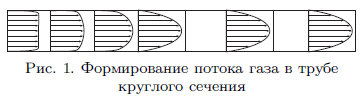
\includegraphics[width = 0.6\textwidth]{133_1.png}
  \end{center}
\end{wrapfigure}
При втекании газа в трубку из большого резервуара скорости слоев вначале постоянны по всему сечению (рис. 1). По мере продвижения газа по трубке картина распределения скоростей меняется, так как сила трения о стенку тормозит прилежащие к ней слои. Характерное для ламинарного течения параболическое распределение скоростей устанавливается на некотором расстоянии $a$ от входа в трубку, которое зависит от радиуса трубки $r$ и числа Рейнольдса по формуле
\[a \approx  0,2 r \cdot Re \text{ } \text{ } \text{ } (3)\]
Градиент давления на участке формирования потока оказывается большим, чем на участке с установившимся ламинарным течением, что позволяет разделить эти участки экспериментально. Формула (3) дает возможность оценить длину участка формирования.
\subsection*{Экспериментальная установка}
\begin{center}
    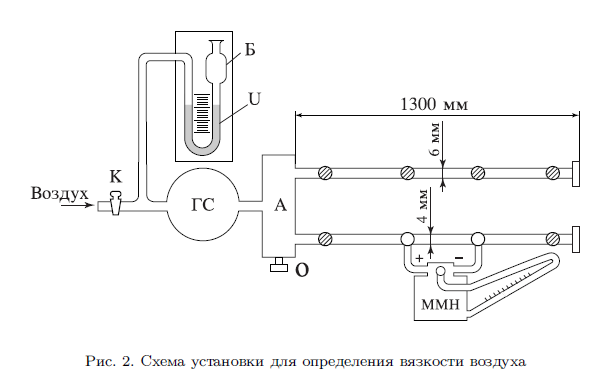
\includegraphics[width = \textwidth]{133_2.png}
  \end{center}
  Измерения производятся на экспериментальной установке, схема которой изображена на рис. 2. Поток воздуха под давлением, несколько превышающим атмосферное (на 5-7 см вод. ст.), через газовый счетчик ГС поступает в резервуар А, к которому припаяны тонкие металлические трубки. Примерные размеры трубок указаны на рисунке (точные размеры обозначены на установке). Обе трубки на концах снабжены заглушками, не пропускающими воздух. Во время измерений заглушка открывается только на рабочей трубке; конец другой трубки должен быть плотно закрыт. Перед входом в газосчётчик поставлена U-образная трубка, наполовину заполненная водой. Она выполняет две задачи. Первая - измерение давления газа на входе в газосчётчик. Вторая - предохранение газосчётчика от выхода из строя. Дело в том, что газосчётчик устойчиво работает, если давление газа на его входе не превышает 600 мм водяного столба. Высота U-образной трубки примерно 600 мм, поэтому, когда давление на входе в счётчик превышает 600 мм водяного столба,вода из U-образной трубки выплёскивается в защитный баллон Б и, создавая шум, привлекает к себе внимание экспериментатора. 
\section*{Ход работы}
\begin{enumerate}
\item Подготавливаем установку к работе: устанавливаем приборы по уровням, проверяем наличие воды в газовом счетчике по водомерному устройству, установливаем на ноль мениск микроманометра. Полный объём измерения проводим на одной из трубок (лучше на трубке $d = 4$ мм).
\item По формуле (3) оцениваем расстояние, на котором происходит формирование потока при ламинарном течении. Расчет проведим для $Re
= 1000$. $a \approx 0,39$ м
\item Подсоединяем микроманометр к двум соседним выводам выбранной трубки на участке со сформировавшимся потоком. Отвинчиваем пробку на конце этой трубки; все остальные выводы на трубках плотно завинчены пробками, снабженными резиновыми прокладками.
\item Медленно открывая кран К (рис. 2) и впуская воздух в установку, внимательно следим за показаниями микроманометра. При больших перепадах давления спирт может вылиться из микроманометра через трубку 11.
\item Измеряем вязкость воздуха. Для этого снимаем зависимость разности давлений $\Delta P$ от расхода воздуха $Q =\Delta V/ \Delta t$, при этом $\Delta V$ измеряется газовым счетчиком, а $\Delta t$ секундомером. Устанавливаем множитель на стойке 4 равным 0,2. Начинаем с малых перепадов давлений (2-3 мм вод. ст.), постепенно увеличивая расход $Q$. В диапазоне от 0 до 100 дел. по шкале 2 должно быть не менее 5-6 точек замера. Это необходимо для того, чтобы заведомо попасть в режим ламинарного течения. После этого замеры можно проводить реже, но в более широком диапазоне по давлению, чтобы попасть в турбулентный режим. По полученным данным строим график $\Delta P = f(Q)$. Из формулы (2) видно, что при ламинарном потоке зависимость $\Delta P$ от $Q$ должна быть линейной. При возникновении турбулентности линейность графика нарушается: разность давлений растет быстрее, чем расход.
\item По угловому коэффициенту прямолинейного участка графика определяем вязкость воздуха $\eta = \dfrac{\pi r^4}{8l} \dfrac{\Delta P}{Q_V}$, где $l = (91 \pm 1)$ см, $r = (1,95 \pm 0,03)$ мм, $\dfrac{\Delta P}{\Delta Q} = (1865000 \pm 107000)$ $\text{Па} \cdot c / \text{м}^3$. Итак $\eta = (1900 \pm 100)10^{-8} \text{ Па} \cdot \text{с}$

\begin{tabular}{|c|c|c|c|}
\hline
$P, \text{ Па}$ & $\sigma_P, \text{ Па}$ & $Q, \text{ л/с}$ & $\sigma_Q, \text{ л/с}$ \\ \hline
43 & 2 & 0,0268 & 0,0003 \\ \hline
73 & 2 & 0,044 & 0,002 \\ \hline
94 & 2 & 0,057 & 0,003 \\ \hline
108 & 2 & 0,063 & 0,004 \\ \hline
131 & 2 & 0,072 & 0,005 \\ \hline
180 & 2 & 0,094 & 0,009 \\ \hline
147 & 2 & 0,081 & 0,007 \\ \hline
216 & 2 & 0,102 & 0,002 \\ \hline
274 & 2 & 0,111 & 0,002 \\ \hline
249 & 2 & 0,11 & 0,01 \\ \hline
333 & 2 & 0,13 & 0,02 \\ \hline
451 & 2 & 0,14 & 0,02 \\ \hline
\end{tabular}

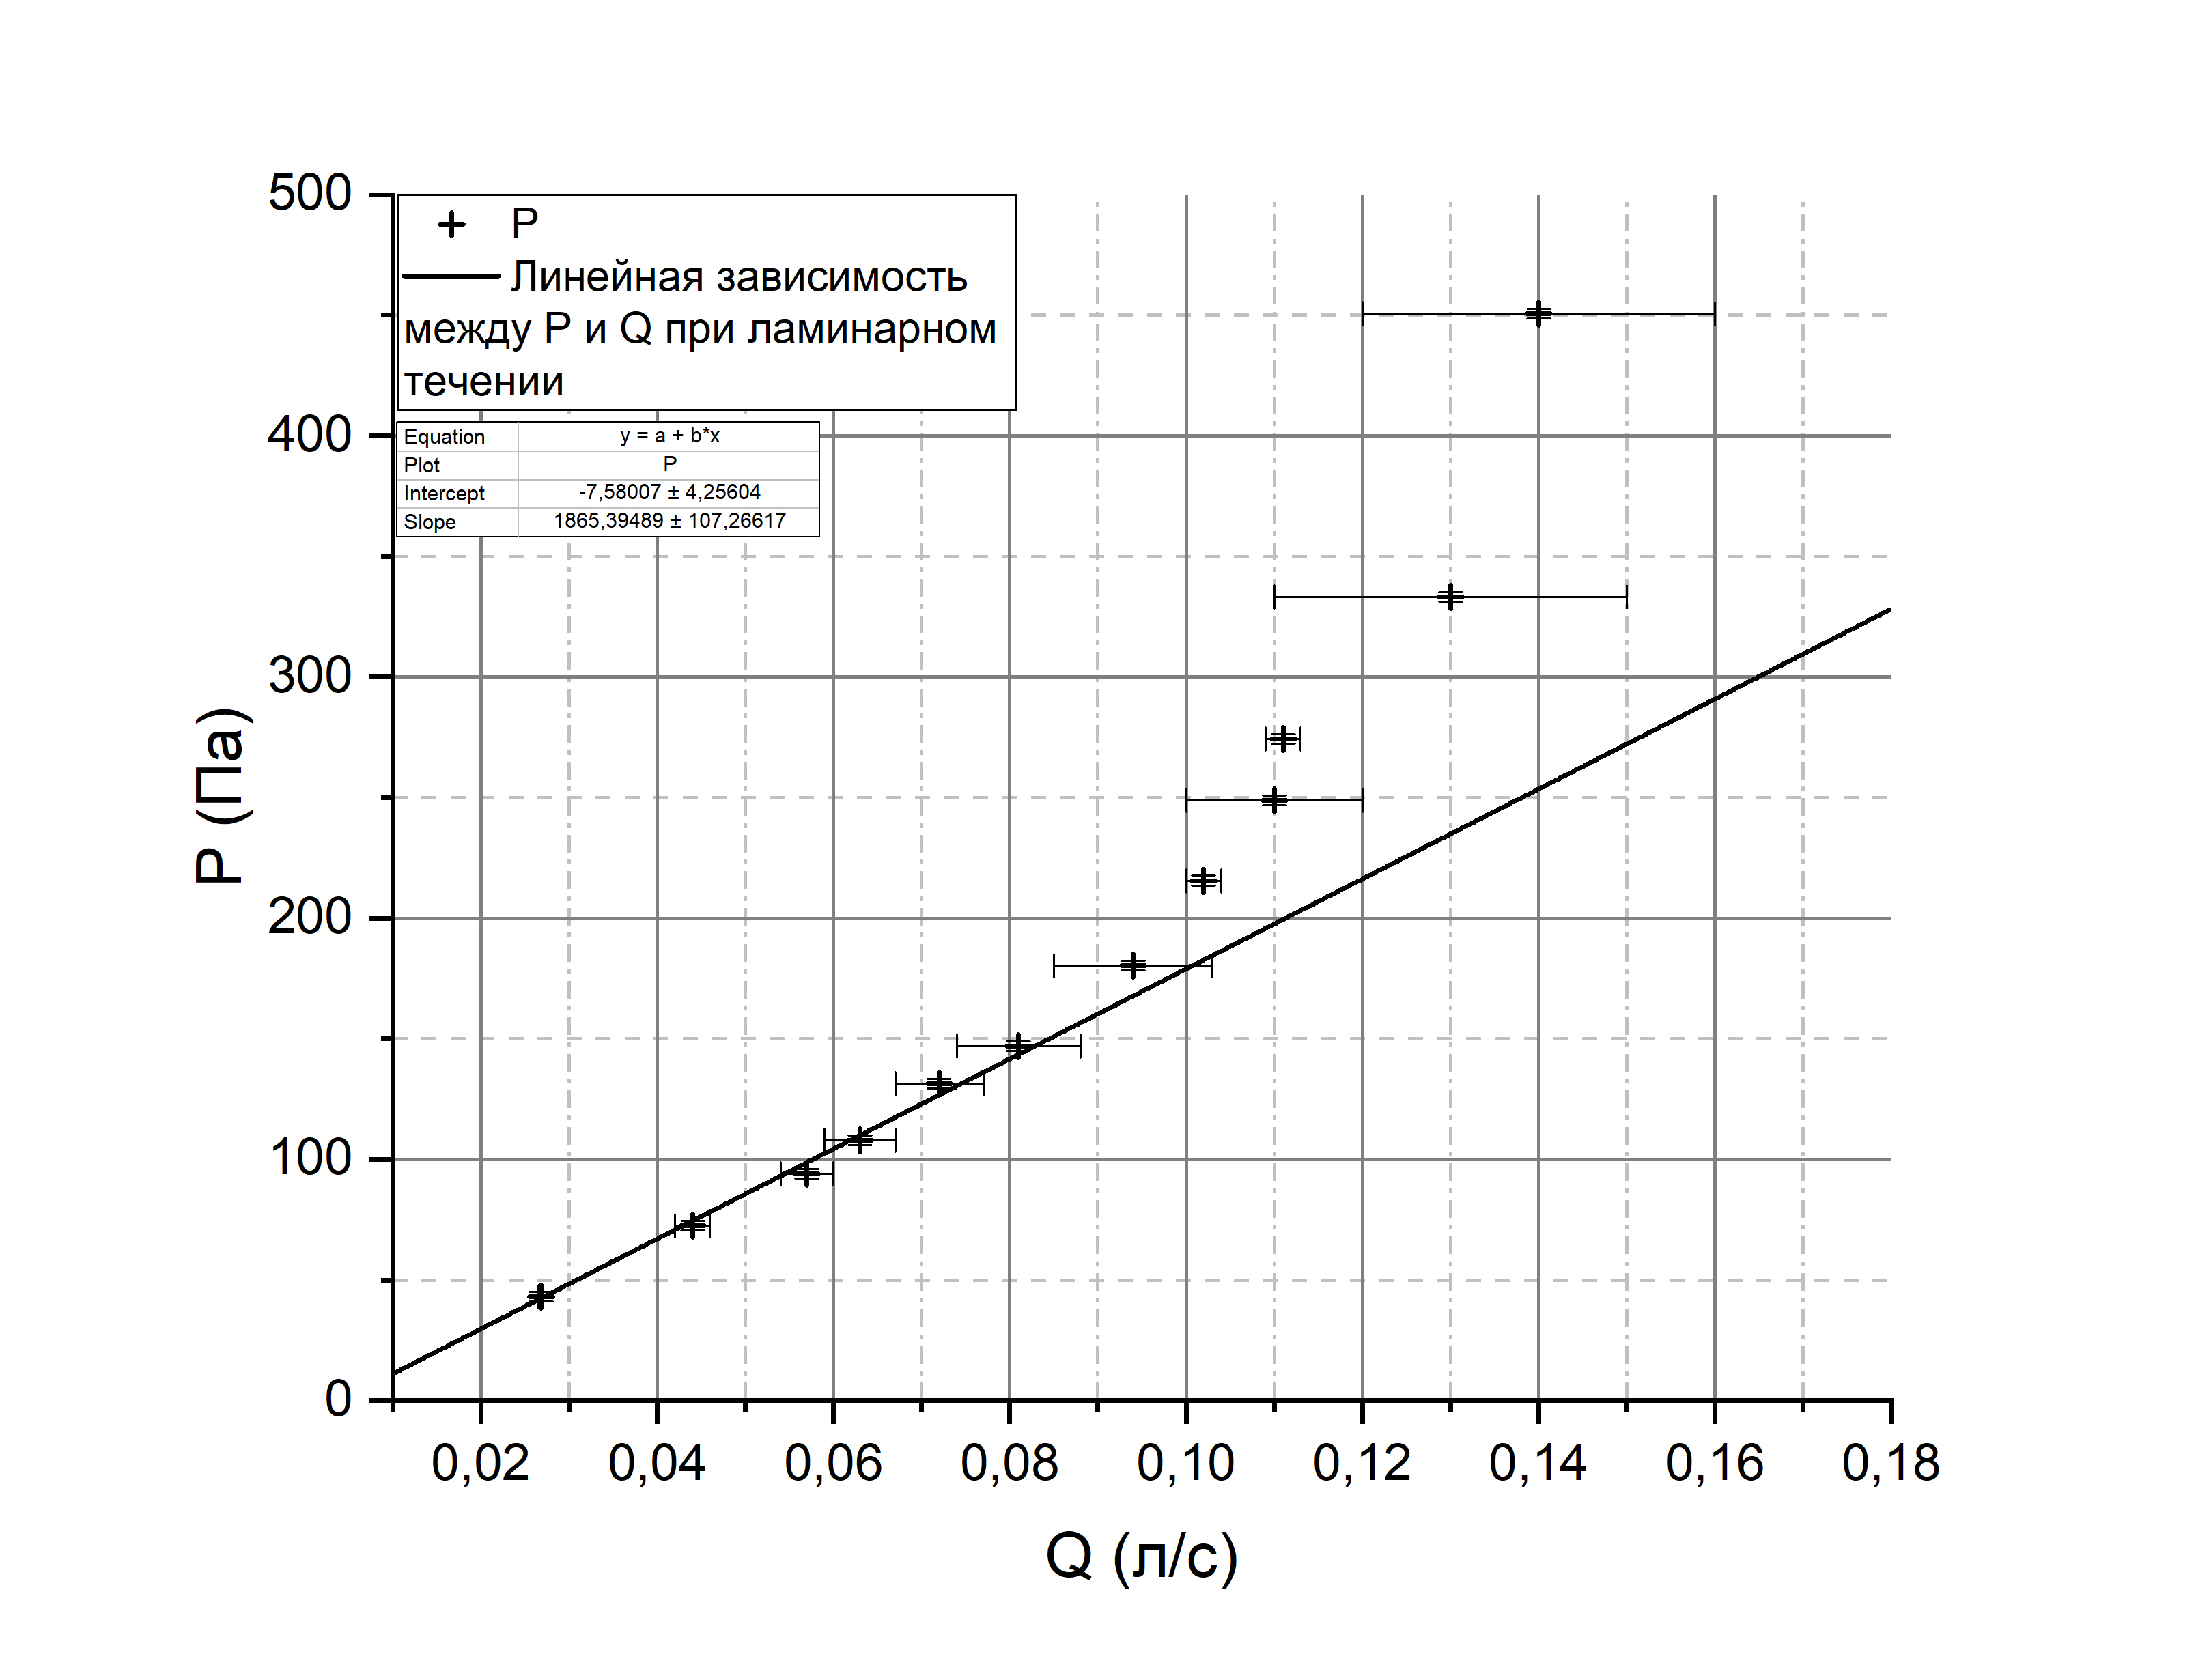
\includegraphics[width = \textwidth]{133_4.jpg}
\item Вычисляем значение числа Рейнольдса $Re \approx (950 \pm 60)$ для переходной области между ламинарным и турбулентным течениями. Что совпаает с табличным значением.
\item При расходе, заведомо обеспечивающем ламинарность потока, измеряем распределение давления вдоль трубки. Для этого микроманометр последовательно подсоединяем ко всем ее выводам, включая и вывод "0" (рис. 2). Строим график зависимости давления от длины вдоль трубки $P = f(l)$. Из графика оцениваем длину участка, на котором происходит установление потока. Сравниваем найденный результат с результатом, вычисленным по формуле (3). Получаем $a \approx 40$ см.

\textbf{для тонкой трубы}

\begin{tabular}{|c|c|c|c|}
\hline
$P, \text{ Па}$ & $\sigma_P, \text{ Па}$ & $l$, м & $\sigma_l$, м \\ \hline
102 & 2 & 1,31 & 0,01 \\ \hline
67 & 2 & 0,81 & 0,01 \\ \hline
37 & 2 & 0,41 & 0,01 \\ \hline
14 & 2 & 0,11 & 0,01 \\ \hline
79 & 2 & 1,2 & 0,01 \\ \hline
59 & 2 & 0,7 & 0,01 \\ \hline
33 & 2 & 0,4 & 0,01 \\ \hline
47 & 2 & 0,5 & 0,01 \\ \hline
20 & 2 & 0,3 & 0,01 \\ \hline
\end{tabular}

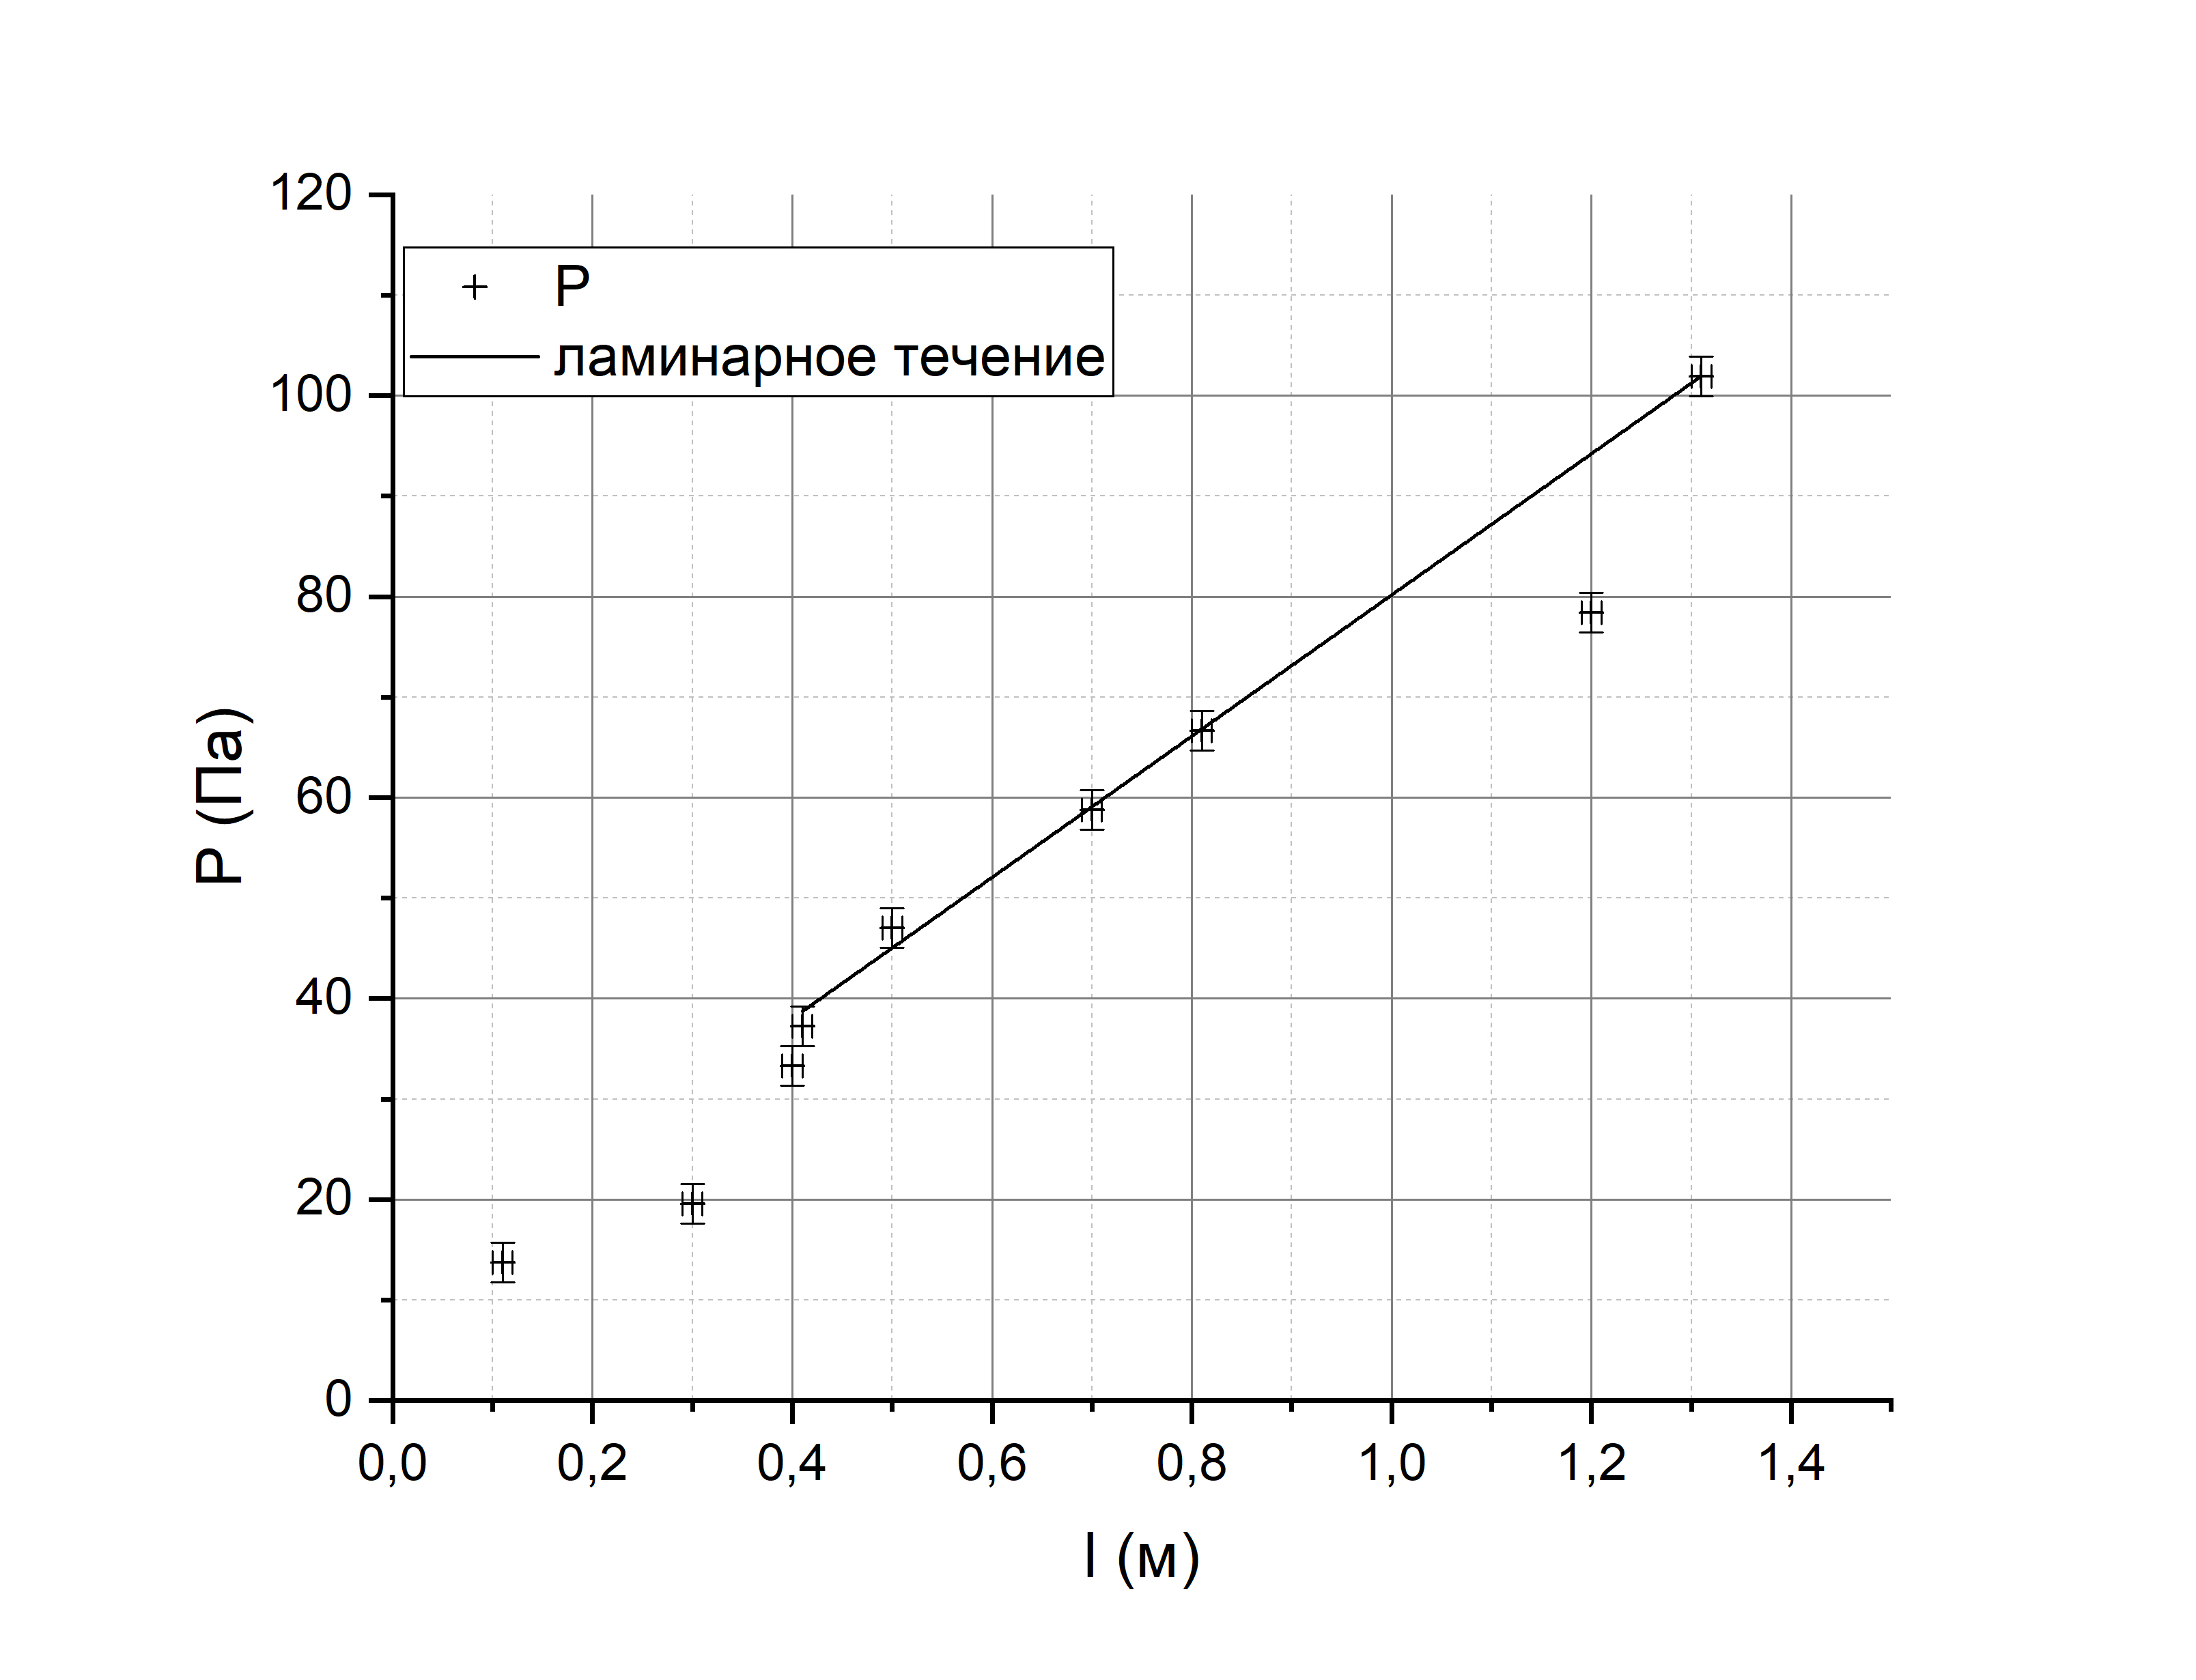
\includegraphics[width = \textwidth]{133_3.jpg}

\newpage
\textbf{для толстой трубы}

\begin{tabular}{|c|c|c|c|}
\hline
$P, \text{ Па}$ & $\sigma_P, \text{ Па}$ & $l$, м & $\sigma_l$, м \\ \hline
49 & 2 & 1,31 & 0,01 \\ \hline
33 & 2 & 0,81 & 0,01 \\ \hline
20 & 2 & 0,41 & 0,01 \\ \hline
12 & 2 & 0,11 & 0,01 \\ \hline
45 & 2 & 1,2 & 0,01 \\ \hline
30 & 2 & 0,7 & 0,01 \\ \hline
16 & 2 & 0,3 & 0,01 \\ \hline
37 & 2 & 0,9 & 0,01 \\ \hline
20 & 2 & 0,4 & 0,01 \\ \hline
\end{tabular}

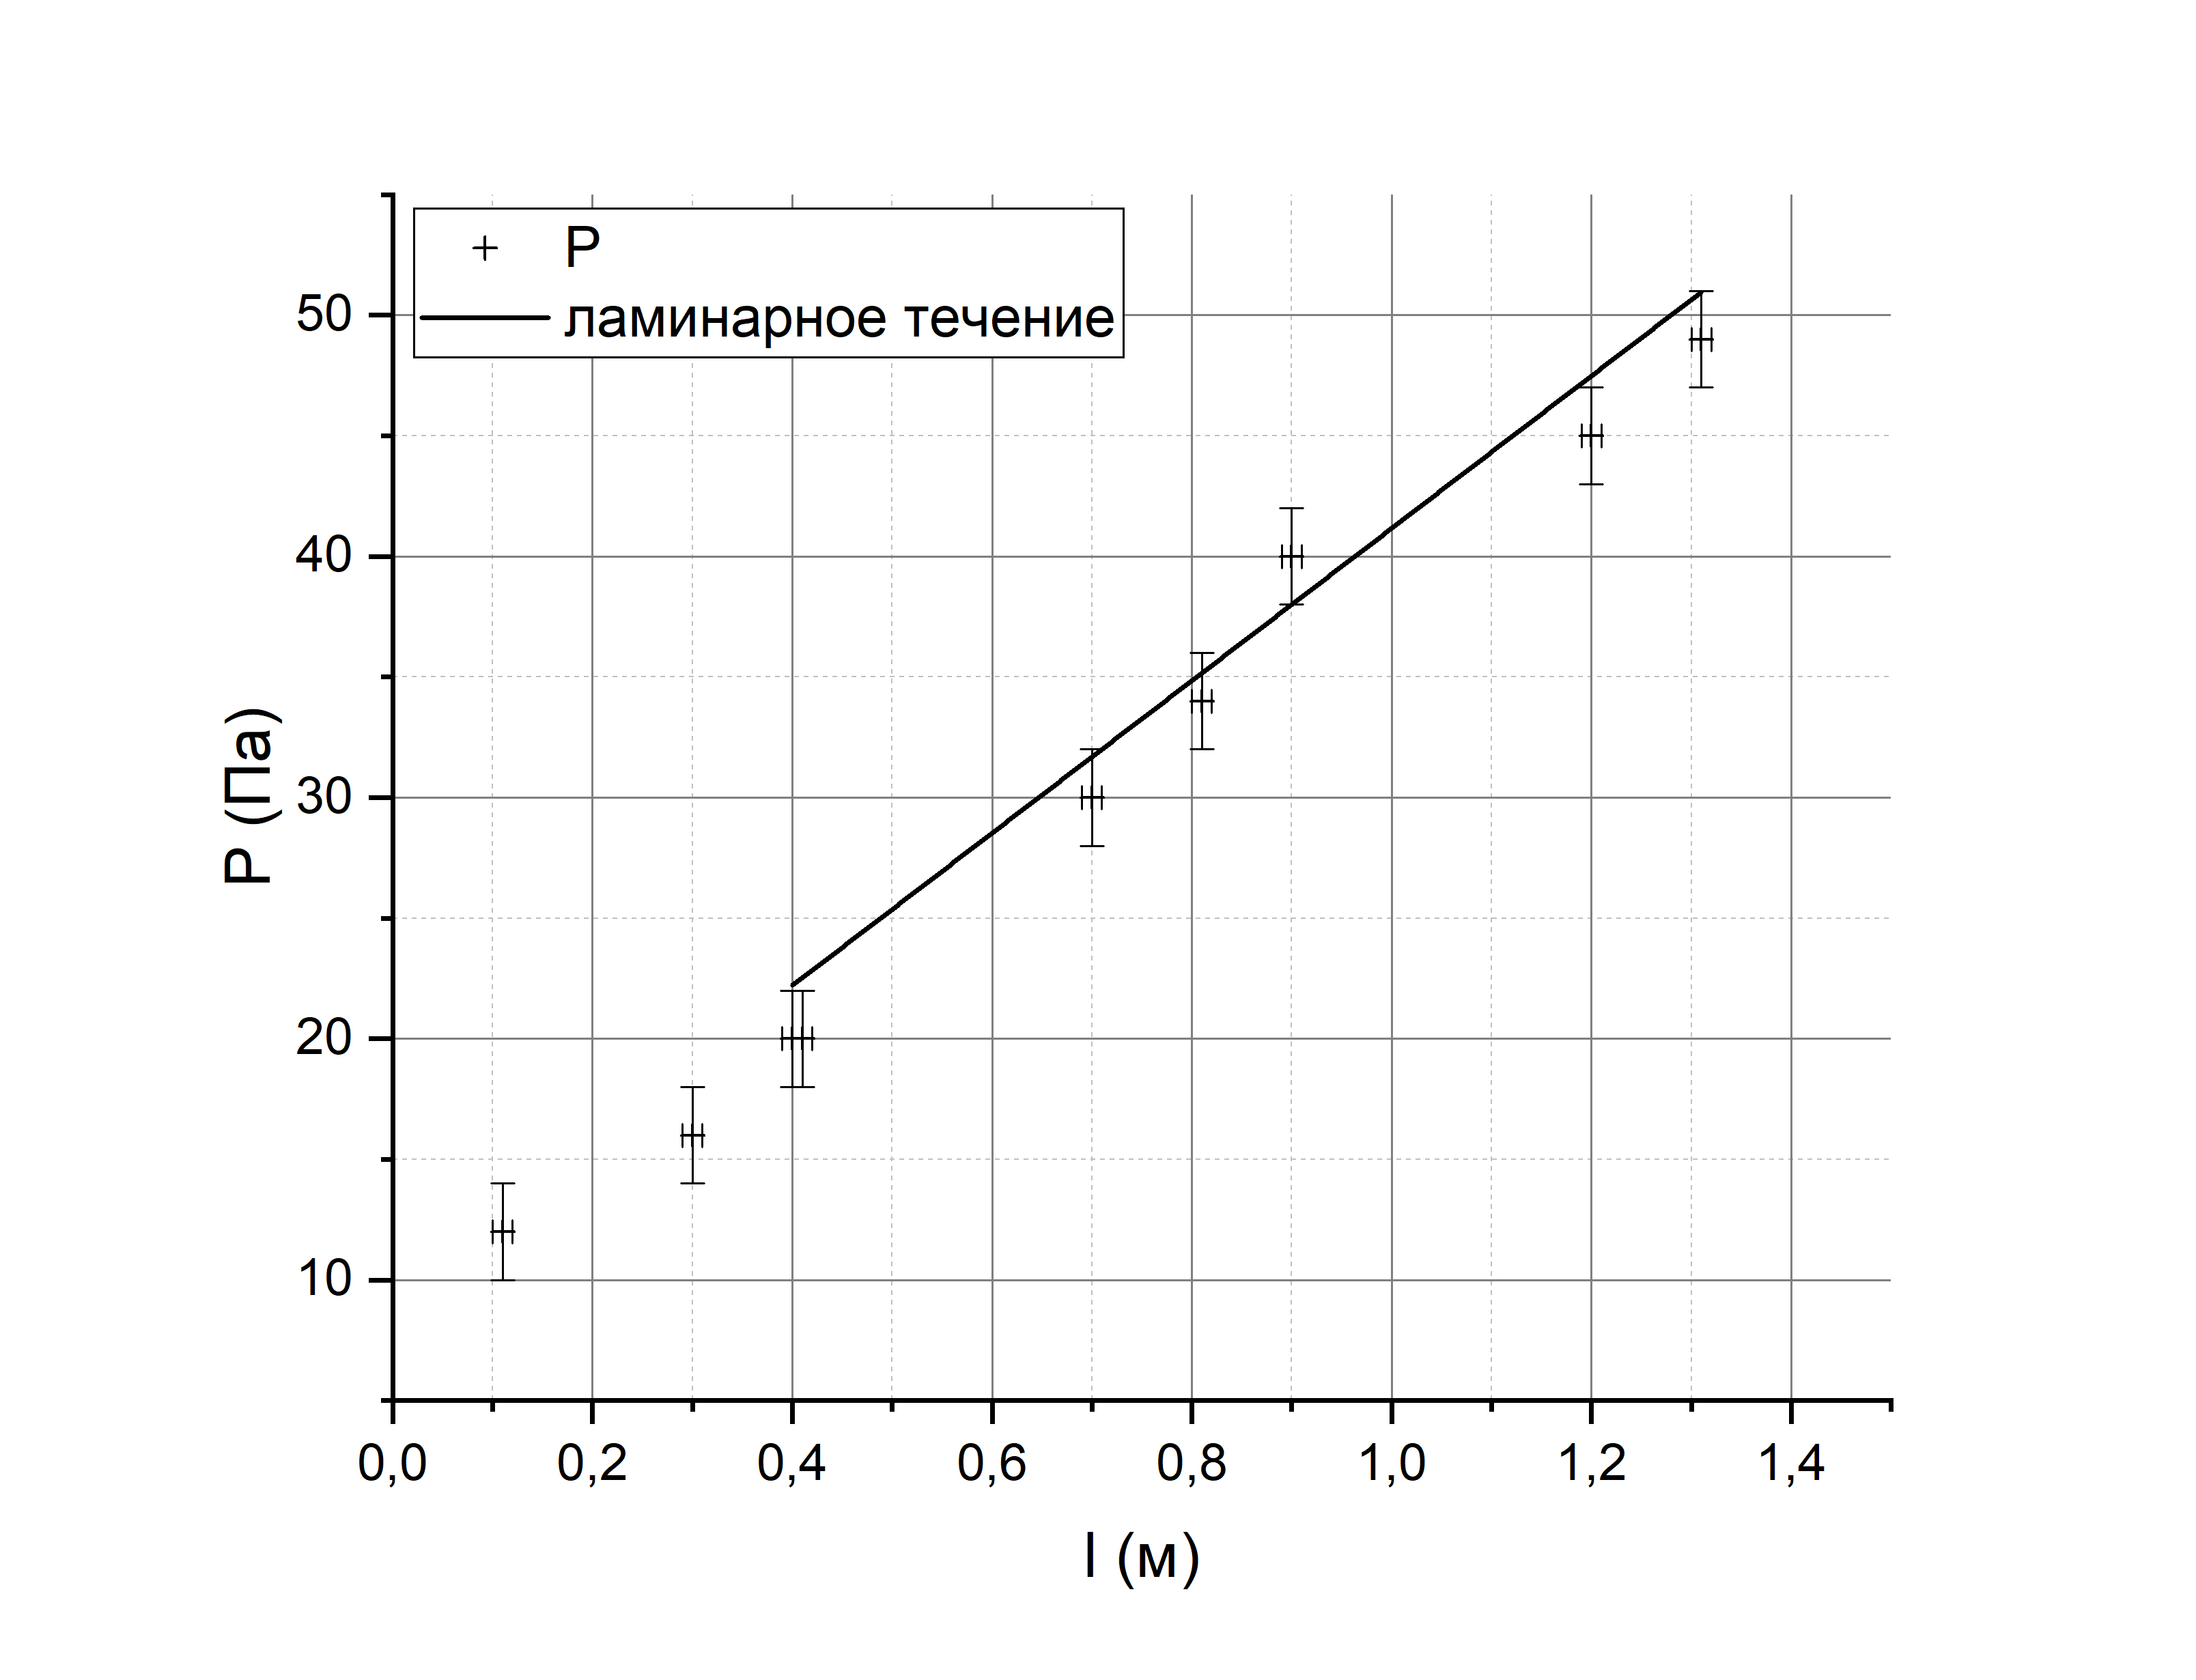
\includegraphics[width = \textwidth]{133_5.jpg}
\item Для всех трубок на участках со сформированным течением (в конце
трубок) в ламинарном режиме ($Re < 500$) снимаем зависимости $Q = f(P)$. Обрабатываем результаты по формуле 
\[\dfrac{8 l \eta Q}{\pi (P_1 - P_2)} = r^n\]
\begin{tabular}{|c|c|c|c|c|c|c|c|}
\hline
\multicolumn{4}{|c|}{$d = (5,25 \pm 0,5)$ мм} & \multicolumn{4}{c|}{$d = (3,9 \pm 0,05)$, мм} \\ \hline
$P$, Па & $\sigma_P$, Па & $q$, л/c & $\sigma_Q$, л/с & $P, \text{ Па}$ & $\sigma_P, \text{ Па}$ & $Q, \text{ л/с}$ & $\sigma_Q, \text{ л/с}$ \\ \hline
59 & 2 & 0,12 & 0,001 & 43,12 & 2 & 0,0268 & 0,0003 \\ \hline
47 & 2 & 0,113 & 0,001 & 72,52 & 2 & 0,044 & 0,002 \\ \hline
29 & 2 & 0,062 & 0,001 & 94,08 & 2 & 0,057 & 0,003 \\ \hline
12 & 2 & 0,022 & 0,001 & 107,8 & 2 & 0,063 & 0,004 \\ \hline
\end{tabular}

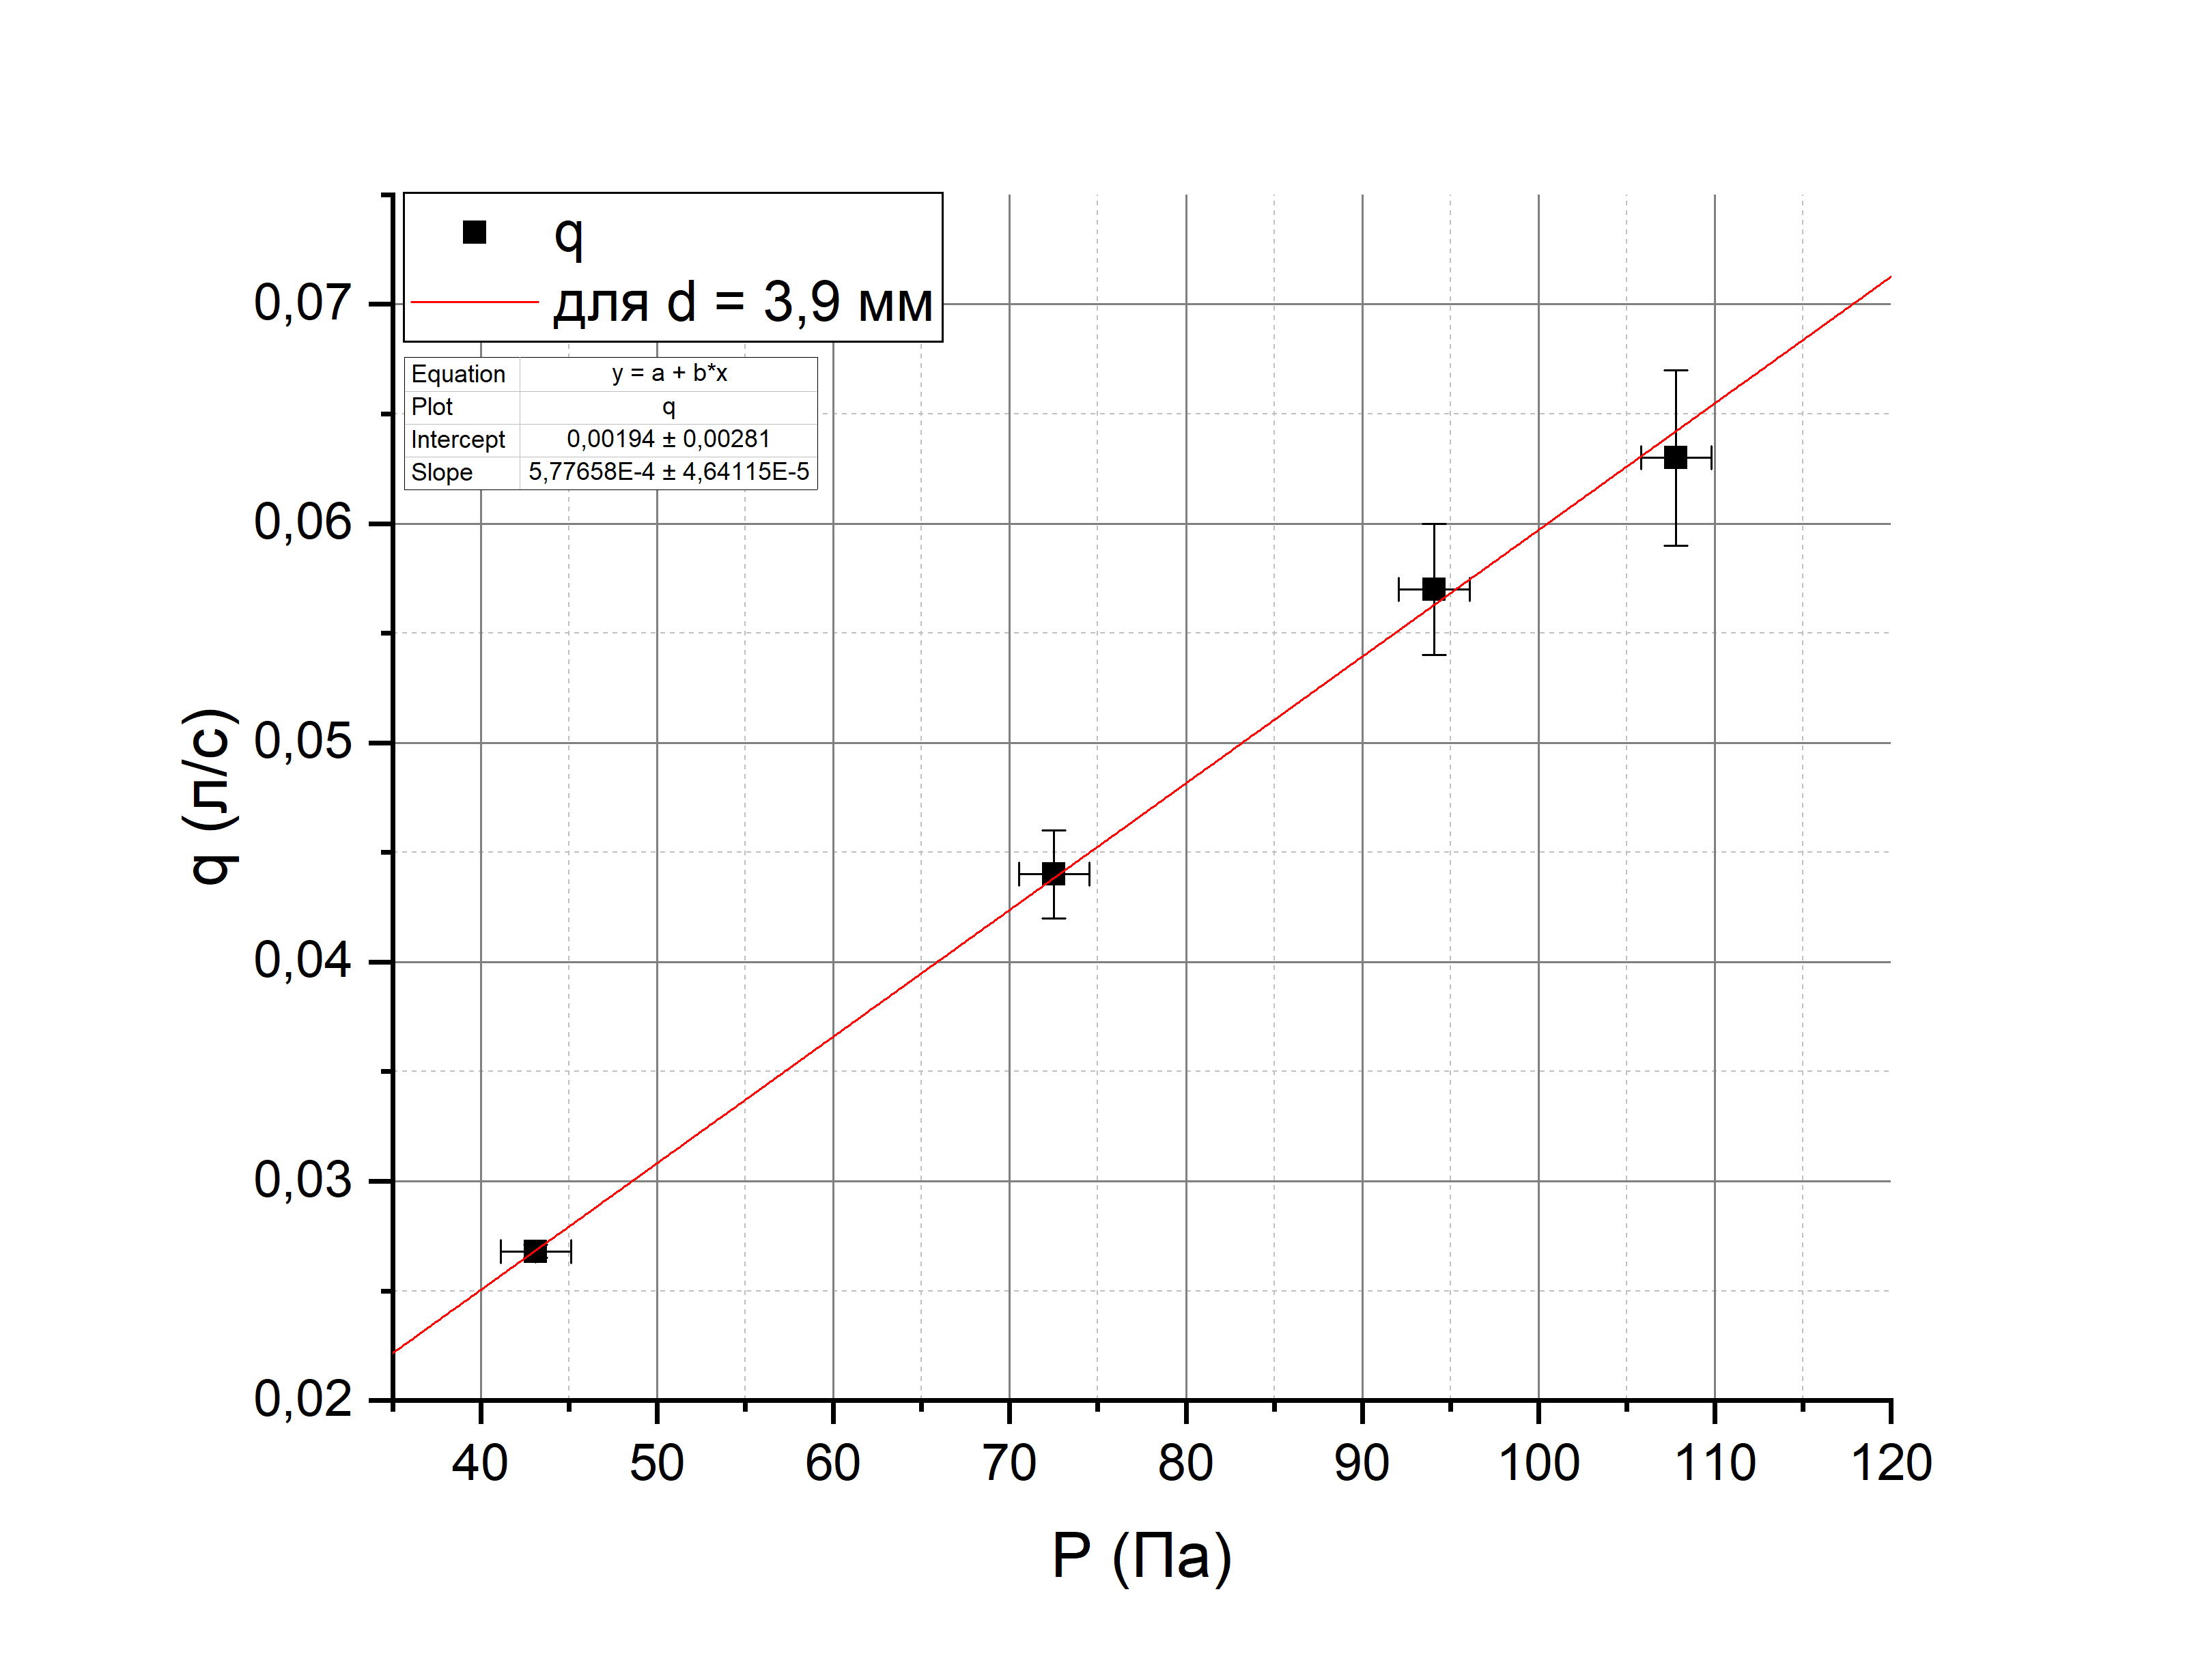
\includegraphics[width = 0.85\textwidth]{133_6.jpg}

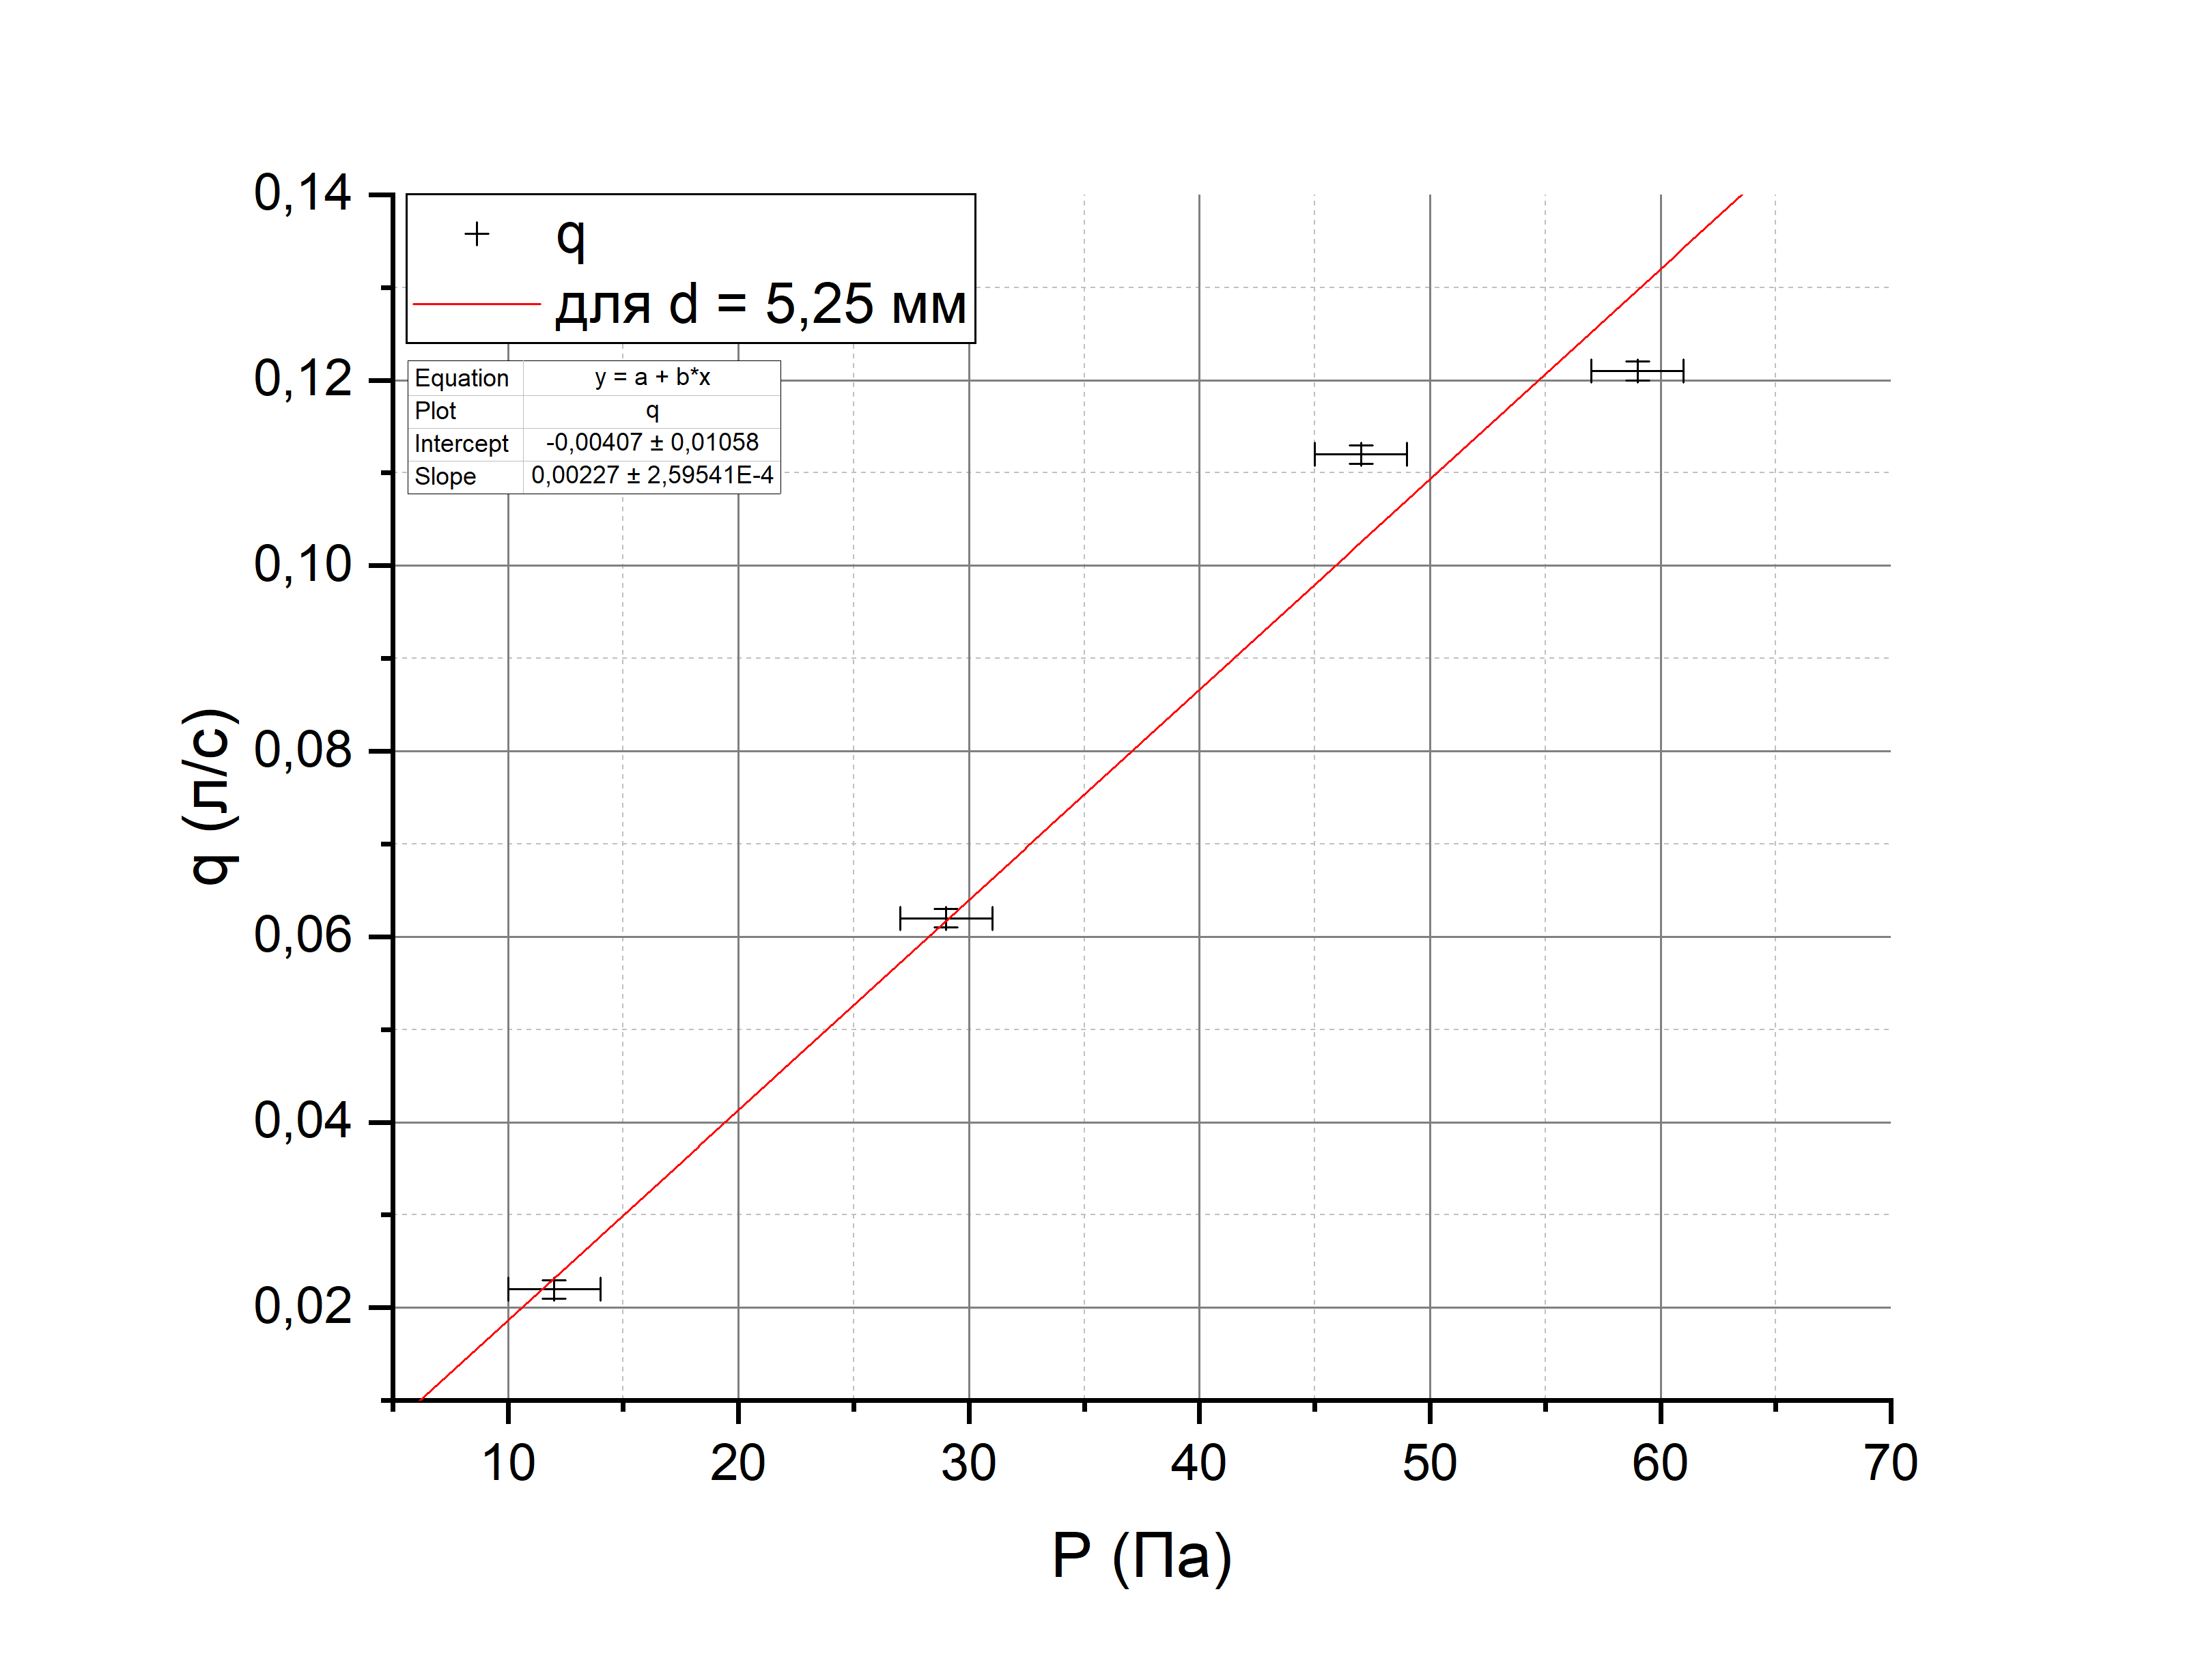
\includegraphics[width = 0.85\textwidth]{133_7.jpg}

Строим график в двойном логарифмическом масштабе, то есть по оси ординат откладываем $\ln \left( \dfrac{8 l \eta Q}{\pi (P_1 - P_2)}\right)$, а по оси абсцисс - $\ln r$. По графику определяем $n \approx 4,5 \pm 0,7$.

Обозначим $\dfrac{8 l \eta Q}{\pi (P_1 - P_2)} = Const$

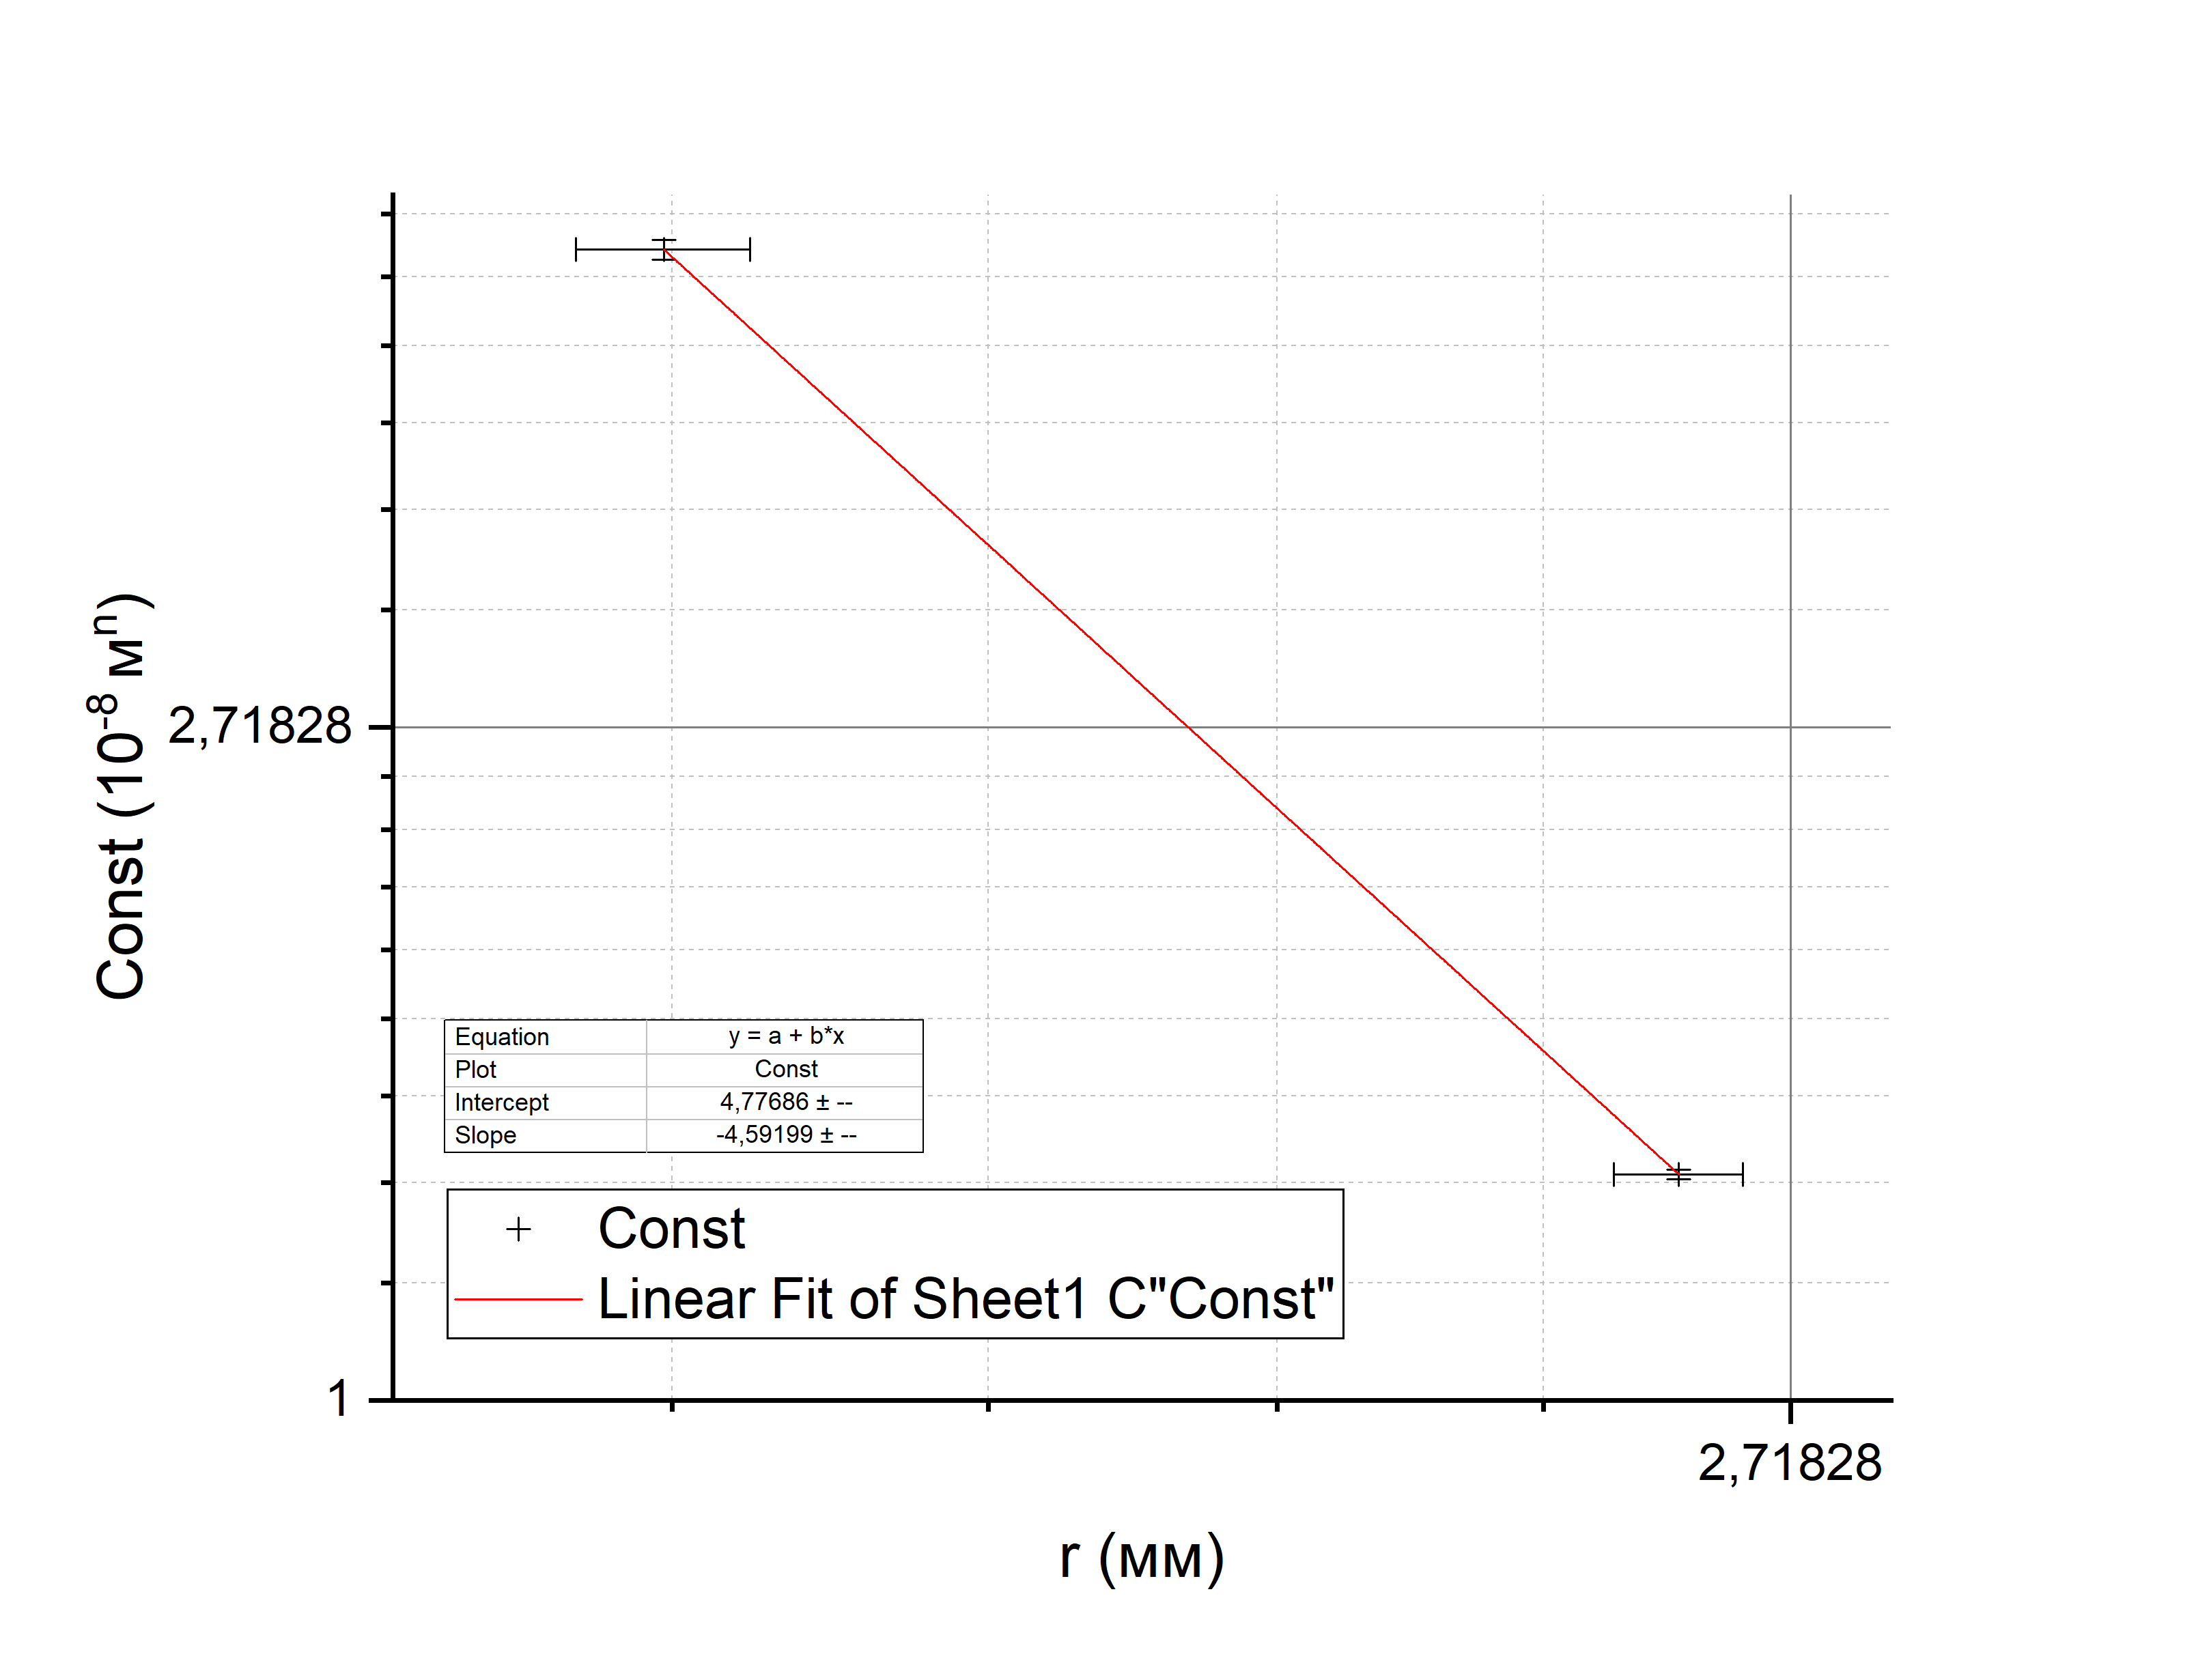
\includegraphics[width = 0.8\textwidth]{133_8.jpg}


\end{enumerate}
\end{document}